% Options for packages loaded elsewhere
\PassOptionsToPackage{unicode}{hyperref}
\PassOptionsToPackage{hyphens}{url}
\PassOptionsToPackage{dvipsnames,svgnames,x11names}{xcolor}
%
\documentclass[
  10pt,
  dvipsnames,enabledeprecatedfontcommands]{scrartcl}
\title{Weight Chapter Outline}
\author{}
\date{\vspace{-2.5em}9/1/2022}

\usepackage{amsmath,amssymb}
\usepackage{lmodern}
\usepackage{iftex}
\ifPDFTeX
  \usepackage[T1]{fontenc}
  \usepackage[utf8]{inputenc}
  \usepackage{textcomp} % provide euro and other symbols
\else % if luatex or xetex
  \usepackage{unicode-math}
  \defaultfontfeatures{Scale=MatchLowercase}
  \defaultfontfeatures[\rmfamily]{Ligatures=TeX,Scale=1}
\fi
% Use upquote if available, for straight quotes in verbatim environments
\IfFileExists{upquote.sty}{\usepackage{upquote}}{}
\IfFileExists{microtype.sty}{% use microtype if available
  \usepackage[]{microtype}
  \UseMicrotypeSet[protrusion]{basicmath} % disable protrusion for tt fonts
}{}
\usepackage{xcolor}
\IfFileExists{xurl.sty}{\usepackage{xurl}}{} % add URL line breaks if available
\IfFileExists{bookmark.sty}{\usepackage{bookmark}}{\usepackage{hyperref}}
\hypersetup{
  pdftitle={Weight Chapter Outline},
  colorlinks=true,
  linkcolor={Maroon},
  filecolor={Maroon},
  citecolor={Blue},
  urlcolor={blue},
  pdfcreator={LaTeX via pandoc}}
\urlstyle{same} % disable monospaced font for URLs
\usepackage{graphicx}
\makeatletter
\def\maxwidth{\ifdim\Gin@nat@width>\linewidth\linewidth\else\Gin@nat@width\fi}
\def\maxheight{\ifdim\Gin@nat@height>\textheight\textheight\else\Gin@nat@height\fi}
\makeatother
% Scale images if necessary, so that they will not overflow the page
% margins by default, and it is still possible to overwrite the defaults
% using explicit options in \includegraphics[width, height, ...]{}
\setkeys{Gin}{width=\maxwidth,height=\maxheight,keepaspectratio}
% Set default figure placement to htbp
\makeatletter
\def\fps@figure{htbp}
\makeatother
\setlength{\emergencystretch}{3em} % prevent overfull lines
\providecommand{\tightlist}{%
  \setlength{\itemsep}{0pt}\setlength{\parskip}{0pt}}
\setcounter{secnumdepth}{5}
\newlength{\cslhangindent}
\setlength{\cslhangindent}{1.5em}
\newlength{\csllabelwidth}
\setlength{\csllabelwidth}{3em}
\newlength{\cslentryspacingunit} % times entry-spacing
\setlength{\cslentryspacingunit}{\parskip}
\newenvironment{CSLReferences}[2] % #1 hanging-ident, #2 entry spacing
 {% don't indent paragraphs
  \setlength{\parindent}{0pt}
  % turn on hanging indent if param 1 is 1
  \ifodd #1
  \let\oldpar\par
  \def\par{\hangindent=\cslhangindent\oldpar}
  \fi
  % set entry spacing
  \setlength{\parskip}{#2\cslentryspacingunit}
 }%
 {}
\usepackage{calc}
\newcommand{\CSLBlock}[1]{#1\hfill\break}
\newcommand{\CSLLeftMargin}[1]{\parbox[t]{\csllabelwidth}{#1}}
\newcommand{\CSLRightInline}[1]{\parbox[t]{\linewidth - \csllabelwidth}{#1}\break}
\newcommand{\CSLIndent}[1]{\hspace{\cslhangindent}#1}
%\documentclass{article}

% %packages
 \usepackage{booktabs}
\usepackage{subcaption}
\usepackage{multirow}
\usepackage{colortbl}
\usepackage{graphicx}
\usepackage{longtable}
\usepackage{ragged2e}
\usepackage{etex}
%\usepackage{yfonts}
\usepackage{marvosym}
\usepackage[notextcomp]{kpfonts}
\usepackage{nicefrac}
\newcommand*{\QED}{\hfill \footnotesize {\sc Q.e.d.}}
\usepackage{floatrow}
%\usepackage[titletoc]{appendix}
%\renewcommand\thesubsection{\Alph{subsection}}

\usepackage[textsize=footnotesize]{todonotes}
\newcommand{\ali}[1]{\todo[color=gray!40]{#1}}
\newcommand{\mar}[1]{\todo[color=blue!40]{#1}}
\newcommand{\raf}[1]{\todo[color=olive!40]{#1}}
%\linespread{1.5}
\newcommand{\indep}{\!\perp \!\!\! \perp\!}


\setlength{\parindent}{10pt}
\setlength{\parskip}{1pt}


%language
\usepackage{times}
\usepackage{t1enc}
%\usepackage[utf8x]{inputenc}
%\usepackage[polish]{babel}
%\usepackage{polski}




%AMS
\usepackage{amsfonts}
\usepackage{amssymb}
\usepackage{amsthm}
\usepackage{amsmath}
\usepackage{mathtools}

\usepackage{geometry}
 \geometry{a4paper,left=35mm,top=20mm,}


%environments
\newtheorem{fact}{Fact}



%abbreviations
\newcommand{\ra}{\rangle}
\newcommand{\la}{\langle}
\newcommand{\n}{\neg}
\newcommand{\et}{\wedge}
\newcommand{\jt}{\rightarrow}
\newcommand{\ko}[1]{\forall  #1\,}
\newcommand{\ro}{\leftrightarrow}
\newcommand{\exi}[1]{\exists\, {_{#1}}}
\newcommand{\pr}[1]{\mathsf{P}(#1)}
\newcommand{\cost}{\mathsf{cost}}
\newcommand{\benefit}{\mathsf{benefit}}
\newcommand{\ut}{\mathsf{ut}}

\newcommand{\odds}{\mathsf{Odds}}
\newcommand{\ind}{\mathsf{Ind}}
\newcommand{\nf}[2]{\nicefrac{#1\,}{#2}}
\newcommand{\R}[1]{\texttt{#1}}
\newcommand{\prr}[1]{\mbox{$\mathtt{P}_{prior}(#1)$}}
\newcommand{\prp}[1]{\mbox{$\mathtt{P}_{posterior}(#1)$}}

\newcommand{\s}[1]{\mbox{$\mathsf{#1}$}}


\newtheorem{q}{\color{blue}Question}
\newtheorem{lemma}{Lemma}
\newtheorem{theorem}{Theorem}



%technical intermezzo
%---------------------

\newcommand{\intermezzoa}{
	\begin{minipage}[c]{13cm}
	\begin{center}\rule{10cm}{0.4pt}



	\tiny{\sc Optional Content Starts}
	
	\vspace{-1mm}
	
	\rule{10cm}{0.4pt}\end{center}
	\end{minipage}\nopagebreak 
	}


\newcommand{\intermezzob}{\nopagebreak 
	\begin{minipage}[c]{13cm}
	\begin{center}\rule{10cm}{0.4pt}

	\tiny{\sc Optional Content Ends}
	
	\vspace{-1mm}
	
	\rule{10cm}{0.4pt}\end{center}
	\end{minipage}
	}
%--------------------






















\newtheorem*{reply*}{Reply}
\usepackage{enumitem}
\newcommand{\question}[1]{\begin{enumerate}[resume,leftmargin=0cm,labelsep=0cm,align=left]
\item #1
\end{enumerate}}

\usepackage{float}

% \setbeamertemplate{blocks}[rounded][shadow=true]
% \setbeamertemplate{itemize items}[ball]
% \AtBeginPart{}
% \AtBeginSection{}
% \AtBeginSubsection{}
% \AtBeginSubsubsection{}
% \setlength{\emergencystretch}{0em}
% \setlength{\parskip}{0pt}






\usepackage[authoryear]{natbib}

%\bibliographystyle{apalike}



\usepackage{tikz}
\usetikzlibrary{positioning,shapes,arrows}

\ifLuaTeX
  \usepackage{selnolig}  % disable illegal ligatures
\fi

\begin{document}
\maketitle

{
\hypersetup{linkcolor=}
\setcounter{tocdepth}{2}
\tableofcontents
}
\hypertarget{introduction}{%
\section{Introduction}\label{introduction}}

Consider two different items of match evidence:\footnote{These are
  stylized after two items of evidence in the notorious Wayne Williams
  case. Probabilities have been slightly but not unrealistically shifted
  to be closer to each other to make a conceptual point. The original
  probabilities were 1/100 for the dog fur, and 29/1148 for Wayne
  Williams' hair.} The suspects dog's fur matches the dog fur found in a
carpet wrapped around one of the bodies (\textsf{dog}). A hair found on
one of the victims matches that of the suspect (\textsf{hair}). What are
the fact-finders to make of this evidence? To start with, some
probabilistic evaluation thereof should be useful.

Accordingly, an expert testifies that the probability of a random
person's hair matching the reference sample is 0.0252613, and it so
happens that the probability of a random dog's hair matching the
reference sample is very close, 0.025641. You assume that the
probabilities of matches if the suspect (respectively, the suspect's
dog) is the source is one, and that these probabilities of a match are
independent of each other conditional on either truth value of the
source hypothesis (\(\mathsf{source}\) and \(\neg \mathsf{source}\)).
Then, to evaluate the total impact of the evidence on the source
hypothesis you calculate: \begin{align*}
\pr{\s{dog}\wedge \s{hair} \vert \neg \s{source}} & = \pr{\s{dog} \vert \neg \s{source}} \times \pr{\s{hair} \vert \neg \s{source}} \\
& =  0.0252613 \times  0.025641 = \ensuremath{6.4772626\times 10^{-4}}
\end{align*} This seems like a low number. To get a better grip on how
this should be interpreted, the expert shows you how the posterior
depends on the prior, given this evidence (Figure
\ref{fig:impactOfPoint}. The posterior of .99 is reached as soon as your
prior is higher than 0.061.

\begin{figure}[H]


\begin{center}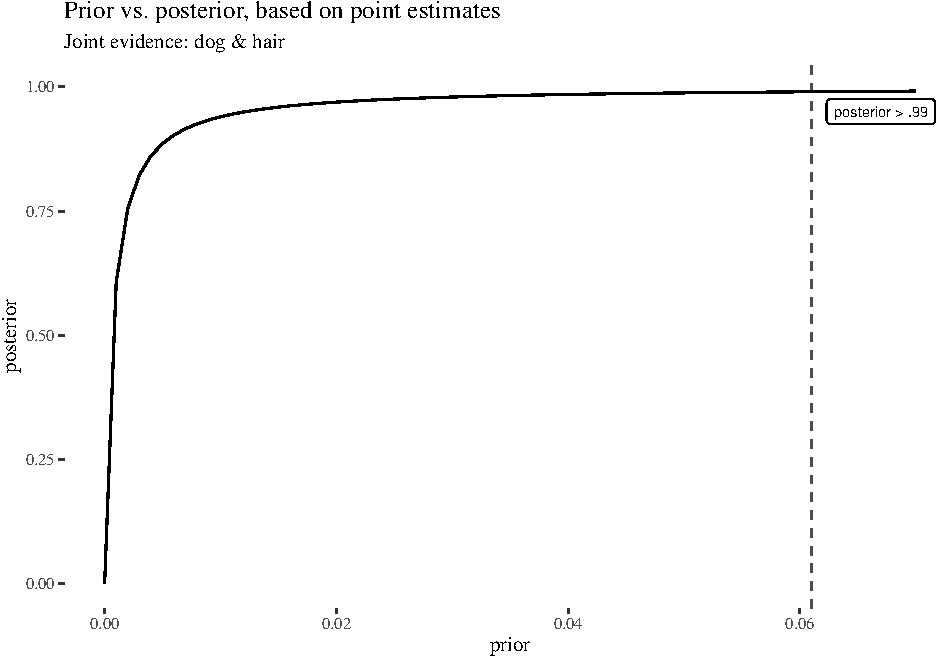
\includegraphics[width=0.8\linewidth]{chapter-outline_files/figure-latex/impactOfPoint4-1} \end{center}

\caption{Impact of dog fur and human hair evidence on the prior, point estimates.}

\label{fig:impactOfPoint}

\end{figure}

While perhaps not sufficient for conviction, the evidence seems pretty
solid: a minor additional piece of evidence could tip the scale. But
then, you reflect on what you have been told and ask the expect:
\emph{wait, but how do you know these exact point probabilities? There must be some aleatory uncertainties around these estimates, and we should pay attention to these!}
The expert agrees, and tells you that in fact the hair evidence estimate
is based on 29 matches found in a database of size 1148, and the dog
evidence estimate was based on finding two matches in a reference class
of size 78.

Well, that means the point estimates did not tell us the whole story,
you think. What to do next? You might try to factor what you have been
just told into your evaluation, but unless you have some training in
probability, you might have hard time doing this correctly. So instead,
you push the expert further:
\emph{well, with a 99\% margin of errors, what are the ranges for these estimates, what are the worst-case and best-case scenarios?}
The expert thinks for a while about giving you confidence intervals, but
abandons this idea, as they are deeply problematic.\footnote{We
  discussed this in a previous chapter XXX.} So instead, he decides to
tell you what the credible intervals are. He says:
\emph{if we start with uniform priors, then the  highest posterior density ranges in which the true frequencies lie with posterior probability of .99 are (.015,.037) for hair and (.002, .103) for fur.}

With good intentions, you calculate the estimate that is the most
charitable to the suspect.
\(\mathsf{P}_{char}(\s{dog}\wedge \s{hair} \vert \neg \s{source}) = .037 * .103 =.003811\).
This number is around 5.88 times greater than the original estimate! You
ask what the impact of evidence on the prior would be given this
scenario, and the answer is that now the prior needs to be higher than
0.274 for the posterior to be above .99 (Figure
\ref{fig:impactOfCharitable}). You are not convinced that the evidence
is fairly strong anymore.

\begin{figure}[H]


\begin{center}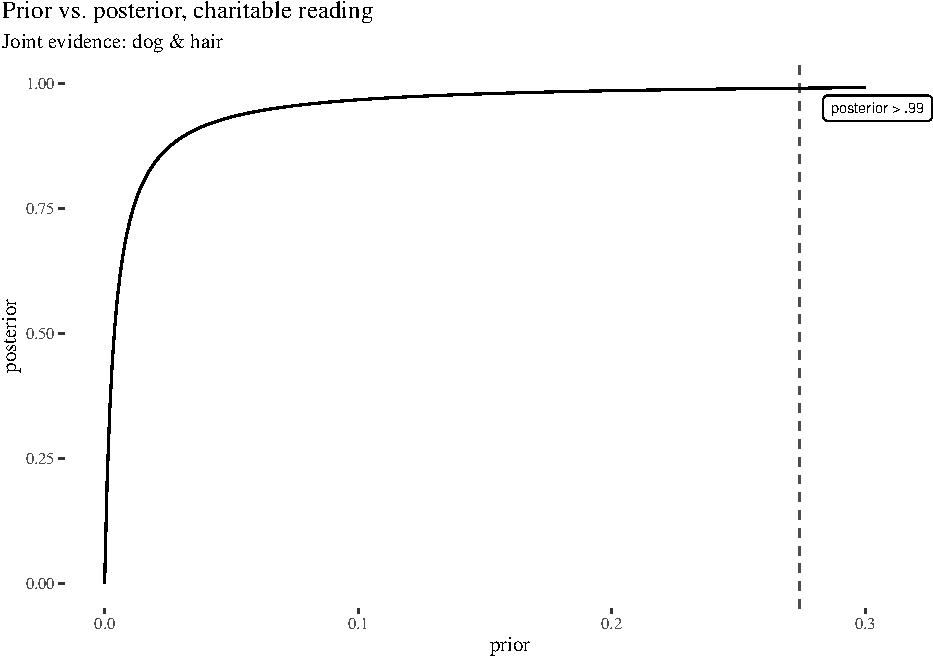
\includegraphics[width=0.8\linewidth]{chapter-outline_files/figure-latex/fig:charitableImpact7-1} \end{center}

\caption{Impact of dog fur and human hair evidence on the prior, charitable reading.}

\label{fig:impactOfCharitable}

\end{figure}

But you made an important blunder. Just because the worst-case
probability estimate for one event is \(x\) and the worst-case
probability estimate for another independent event is \(y\), it does not
follow that the worst-case probability estimate for their conjunction is
\(xy\), if the margin of error is kept fixed. The intuitive reason is
quite simple: just because the probability of an extreme (or larger
absolute) value \(x\) for one variable is .01, and so it is for the
value \(y\) of another independent variable, it does not follow that the
probability that those two independent variables take values \(x\) and
\(y\) simultaneously is the same. This probability is actually much
smaller.

In fact, if you knew what distributions the expert used (it should have
been beta distributions in this context), you could work your way back
and calculate the .99 highest posterior density interval for the
conjunction, which is \((0.000023, 0.002760)\). The proper charitable
reading would then require the prior to be above .215 for the posterior
to be above .99. Still not enough to convict, but at least now we worked
out the consequences of the aleatory uncertainties involved provided the
margin of error is fixed. Is this good enough?

Well, it seems the interval presentation instead of doing us good led us
into error --- the general phenomenon is that intervals do \textbf{not}
contain enough information to reliably reason about such things as
reliability, margins of errors and so on. Even if we are happy with the
interval that we obtained, we won't be able to correctly obtain a new
interval once a new item of evidence is included. That is, unless we
proceed through the densities.

Another problem is that looking at intervals might be useful if the
underlying distributions are fairly symmetrical. But in our case, they
might not be. For instance, Figure \ref{fig:densities} illustrates are
the beta densities for dog fur and human hair, together with
sampling-approximated density for the joint evidence. Crucially, the
distribution is not symmetric, and so switching the margin of error
moves the right edge of the interval much faster towards lower values.
If you were only informed about the edges of the interval, you would be
oblivious to such phenomena and the fact that the most likely value does
\textbf{not} simply lie in the middle between the edges of the interval.

\begin{figure}[H]


\begin{center}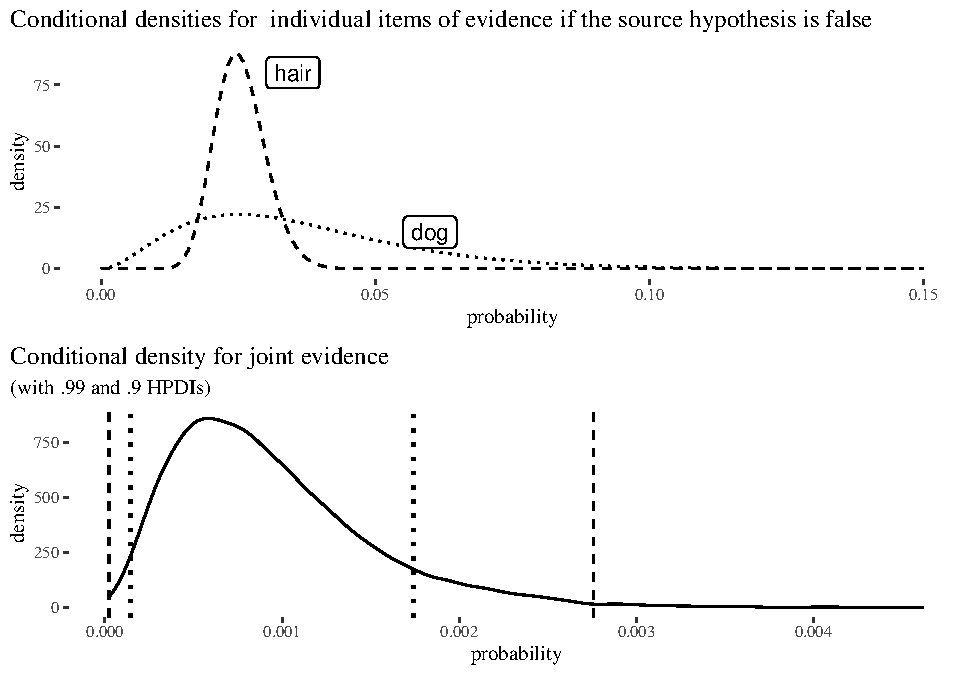
\includegraphics[width=0.8\linewidth]{chapter-outline_files/figure-latex/fig:densities-1} \end{center}

\caption{Beta densities for individual items of evidence and the resulting joint density with .99 and .9 highest posterior density intervals, assuming the sample sizes as discussed and independence, with uniform priors.}

\label{fig:densities}

\end{figure}

This means that a better representation of the uncertainty involving the
dependence of the posterior on the prior involves multiple possible
lines whose density mirrors the density around the probability of the
evidence (Figure \ref{fig:lines}).

\begin{figure}[H]


\begin{center}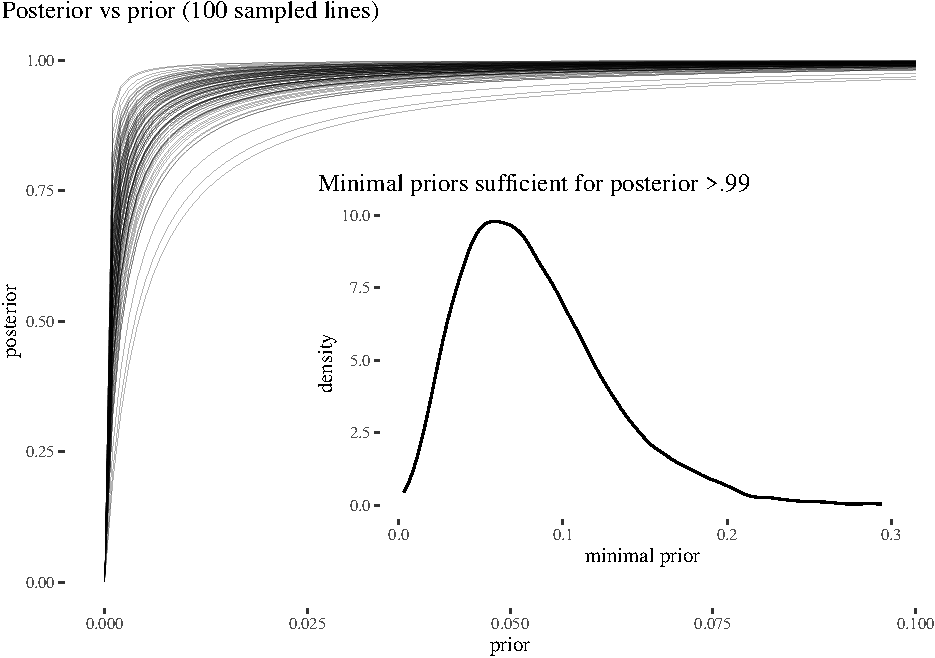
\includegraphics[width=0.8\linewidth]{chapter-outline_files/figure-latex/fig:lines3-1} \end{center}

\caption{100 lines illustrating the uncertainty about the dependence of the posterior on the prior given aleatory uncertainty about the evidence, with the distribution of the minimal priors required for the posterior to be above .99.}

\label{fig:lines}

\end{figure}

\todo{Revise this structure description once the chapter is done}

This is the gist of our chapter: whenever honest density estimates are
available (and they should be available for match evidence evaluation
methods whose reliability has been properly studied), it is those
densities that should be reported and used in further reasoning. This
avoids hiding actual aleatory uncertainties under the carpet, and allows
for more correct reasoning where interval-based representation might
either lead one astray or leave one oblivious to important probabilistic
considerations.

The rest of this chapter expands on this idea in a few dimensions.
First, it places it in the context of philosophical discussions
surrounding a proper probabilistic representation of uncertainty. The
main alternatives on the market are precise probabilism and imprecise
probabilism. We argue that both options are problematic and should be
superseded by the second-order representation whenever possible. Second,
having gained this perspective, we visit a recent discussion in the
forensic science literature, where a prominent proposal is that the
experts, even if they use densities, should integrate and present only
point estimates to the fact-finders. We disagree. Third, we explain how
the approach can be used in more complex situations in which multiple
items of evidence and multiple propositions interact---and the idea is
that such complexities can be handled by sampling from distributions and
approximating densities using multiple Bayesian Networks in the
calculations. Last but not least, we turn to the notion of weight of
evidence. Having distinguished quite a few notions in the vicinity, we
explain how the framework we propose allows for a more successful
explication and implementation of the notion of weight of evidence than
the ones currently available on the market.

\hypertarget{three-probabilisms}{%
\section{Three probabilisms}\label{three-probabilisms}}

This section outlines three version of probabilism: precise, imprecise
and higher-order. Precise probabilism, as the name suggests, posits that
an agent' credal state is modeled by a single, precise probability
measure. Imprecise probabilism replaces precise probabilities by sets of
probability measures, while higher-order probabilism relies on
distributions over parameter values. There are good reasons to abandon
precise probabilism and endorse higher-order probabilism. Imprecise
probabilism is a step in the right direction, but as we will see, it
suffers from too many difficulties of its own.

\hypertarget{precise-probabilism}{%
\subsection{Precise Probabilism}\label{precise-probabilism}}

\textbf{Precise probabilism} (\textsf{PP}) holds that a rational agent's
uncertainty about a hypothesis \(H\) is to be represented as a single,
precise probability measure. This is an elegant and simple theory. But
representing our uncertainty about a proposition in terms of a single,
precise probability runs into a number of difficulties. Precise
probabilism fails to capture an important dimension of how our
uncertainty connects with the evidence we have or have not obtained.
Consider the following simple examples (we will be using examples with
coins for a bit, but the points are general and hold for all sampling
based frequency estimation methods, including those of random match
probability for various pieces of forensic evidence):

\begin{quote}
\textbf{No evidence v. fair coin}
You are about to toss a coin, but have no evidence 
whatsoever about its bias. You are completely ignorant. Sticking to \s{PP} you  follow the principle of insufficient evidence and assign probability .5 to the outcome being \emph{heads}.  Compare this to the situation  in which you know the coin is fair. Sticking to PP, you assign the same probability to the outcome of the next toss being \emph{heads}. 
\end{quote}

\begin{quote}
\textbf{Learning from ignorance}
You start  tossing the former coin, toss it ten times and observe \emph{heads} five times. You started with your bias estimate at .5, but you also end with your bias estimate at .5. Clearly, you have learned something, but whatever that is, it is not captured in the representaiton recommended by \s{PP}.
\end{quote}

\noindent Clearly, precise probabilism has difficulties modeling such
situations.\footnote{Examples of this sort date back to C. S. Peirce,
  who in his 1872 manuscript `The Fixation of Belief' (W3 295) comments:
  ``when we have drawn a thousand times, if about half {[}of the
  beans{]} have been white, we have great confidence in this result
  \ldots{} a confidence which would be entirely wanting if, instead of
  sampling the bag by 1000 drawings, we had done so by only two.'\,'
  Similar remarks can be found in Peirce's 1878
  \emph{Probability of Induction}. There, he also proposes to represent
  uncertainty by at least two numbers, the first depending on the
  inferred probability, and the second measuring the amount of knowledge
  obtained; as the latter, Peirce proposed to use some
  dispersion-related measure of error (but then suggested that an error
  of that estimate should also be estimated and so, so that ideally more
  numbers representing errors would be needed).} The examples suggest
that precise probabilism is not appropriately responsive to evidence. It
ends up assigning a probability of .5 to situations in which one's
evidence is quite different: when no evidence is available about the
coin's bias; when there is little evidence that the coin is fair (say,
after only 2 draws); when there is strong evidence that the coin is fair
(say, after 1000 draws).\footnote{Precise probabilism suffers from other
  difficulties. For example, it has problems with formulating a sensible
  method of probabilistic opinion aggregation Stewart \& Quintana
  (2018). A seemingly intuitive constraint is that if every member
  agrees that \(X\) and \(Y\) are probabilistically independent, the
  aggregated credence should respect this. But this is hard to achieve
  if we stick to \s{PP} (Dietrich \& List, 2016). For instance, a
  \emph{prima facie} obvious method of linear pooling does not respect
  this. Consider probabilistic measures \(p\) and \(q\) such that
  \(p(X) = p(Y) = p(X\vert Y) = 1/3\) and
  \(q(X) = q(Y) = q(X\vert Y) = 2/3\). On both measures, taken
  separately, \(X\) and \(Y\) are independent. Now take the average,
  \(r=p/2+q/2\). Then \(r(X\cap Y) = 5/18 \neq r(X)r(Y)=1/4\).}

\hypertarget{imprecise-probabilism}{%
\subsection{Imprecise Probabilism}\label{imprecise-probabilism}}

What if we give up the assumption that probability assignments should be
precise? \textbf{Imprecise probabilism} (\textsf{IP}) holds that an
agent's credal stance towards a hypothesis \(H\) is to be represented by
means of a \emph{set of probability measures}, typically called a
representor \(\mathbb{P}\), rather than a single measure \(\mathsf{P}\).
The representor should include all and only those probability measures
which are compatible (in a sense to be specified) with the evidence. For
instance, if an agent knows that the coin is fair, their credal state
would be captured by the singleton set \(\{\mathsf{P}\}\), where
\(\mathsf{P}\) is a probability measure which assigns \(.5\) to
\emph{heads}. If, on the other hand, the agent knows nothing about the
coin's bias, their credal state would rather be represented as the set
of all probabilistic measures, as none of them is excluded by the
available evidence. Note that the set of probability measures does not
represent admissible options that the agent could legitimately pick
from. Rather, the agent's credal state is essentially imprecise and
should be represented by means of the entire set of probability
measures.\footnote{For the development of imprecise probabilism, see
  (Fraassen, 2006; Gärdenfors \& Sahlin, 1982; Joyce, 2005; Kaplan,
  1968; Keynes, 1921; Levi, 1974; Sturgeon, 2008; Walley, 1991),
  (Bradley, 2019) is a good source of further references.}

Imprecise probabilism, at least \emph{prima facie}, offers a
straightforward picture of learning from evidence, that is a natural
extension of the classical Bayesian approach. When faced with new
evidence \(E\) between time \(t_0\) and \(t_1\), the representor set
should be updated point-wise, running
the\todo{REF Kyburg. Probability and the Logic of Rational Belief. Wesleyan University Press, Middletown Connecticut, 1961 and H. E. Kyburg and C. M. Teng. Uncertain Inference. Cambridge University Press, Cambridge, 2001.}
standard Bayesian updating on each probability measure in the
representor:\footnote{Imprecise probabilism shares some similarities
  with what we might call \textbf{interval probabilism} due to {[}KYBURG
  1961{]}. On interval probabilism, precise probabilities are replaced
  by intervals of probabilities. On imprecise probabilism, instead,
  precise probabilities are replaced by sets of probabilities. This
  makes imprecise probabilism more general, since the probabilities of a
  proposition in the representor set do not have to form a closed
  interval. Moreover, learning on Kyburg's approach is somewhat
  idiosyncratic and is strongly connected to reference classes and
  selection and reshaping rules for intervals. See {[}PEDDEN{]} for a
  introduction. As we have already signaled, as intervals do not contain
  probabilistic information sufficient to guide reasoning with multiple
  propositions and items of evidence, we keep our focus on \s{IP}, which
  is the more promising candidate method.}
\begin{align*} \label{eq:updateRepresentor}
\mathbb{P}_{t_1} = \{\mathsf{P}_{t_1}\vert \exists\, {\mathsf{P}_{t_0} \!\in  \mathbb{P}_{t_0}}\,\, \forall\, {H}\,\, \left[\mathsf{P}_{t_1}(H)=\mathsf{P}_{t_0}(H \vert E)\right] \}.
\end{align*}

The hope is at least that if we start with a range of probabilities that
is not extremely wide, point-wise learning will behave
appropriately.\footnote{The hope is also that \s{IP} offers a feasible
  aggregation method (Elkin \& Wheeler, 2018; Stewart \& Quintana,
  2018): just put all representors together in one set, and voil'a!
  However, this is a very conservative method which quickly leads to
  extremely few points of agreement, and we are not aware of any
  successful practical deployment of this method.} For instance, if we
start with a prior probability of \emph{heads} equal to .4 or .6, then
those measure should be updated to something closer to \(.5\) once we
learn that a given coin has already been tossed ten times with the
observed number of heads equal 5 (call this evidence \(E\)). This would
mean that if the initial range of values was \([.4,.6]\) the posterior
range of values should be more narrow. But even this seemingly
straightforward piece of reasoning is hard to model if we want to avoid
using densities. For to calculate \(\pr{\s{heads}\vert E}\) we need to
calculate \(\pr{E \vert \s{heads}}\pr{\s{heads}}\) and divide it by
\(\pr{E} = \pr{E \vert \s{heads}}\pr{\s{heads}} + \pr{E} = \pr{E \vert \neg \s{heads}}\pr{\neg \s{heads}}\).
The tricky part is obtaining the conditional probabilities
\(\pr{E \vert \s{heads}}\) and \(\pr{E \vert \neg \s{heads}}\) in a
principle manner without explicitly going second-order, estimating the
parameter value and using beta distributions.

The situation is even more difficult if we start with complete lack of
knowledge, as imprecise probabilism runs into the problem of
\textbf{belief inertia} (Levi, 1980). Say you start tossing a coin
knowing nothing about its bias. The range of possibilities is \([0,1]\).
After a few tosses, once you observed at least one tail and at least one
heads, you have excluded the measures assigning 0 or 1 to \emph{heads}.
But what else have you learned? Let's charitably agree that each
particular measure from your initial representor gets updated to one
that is closer to .5, but also now each value in your original interval
can be obtained by updating some \emph{other} measure in your original
representor on the evidence, and the picture does not change no matter
how many observations you have made. For instance, some measure that
initially assigned .4 to \s{heads} might now assign \s{.45} to
\s{heads}, but now a measure that assigned .37 to heads has been updated
to one that assigns \(.4\) to \s{heads}. Thus, if you are to update your
representor point-wise, you will end up with the same representor set.
Consequently, the edges of your resulting interval will remain the same.
In the end, it is not clear how you are supposed to learn that the
proportion of beans is such and such.\footnote{ Here's another example
  from (Rinard, 2013). Either all the marbles in the urn are green
  (\(H_1\)), or exactly one tenth of the marbles are green (\(H_2\)).
  Your initial credence \([0,1]\) in each. Then you learn that a marble
  drawn at random from the urn is green (\(E\)). After conditionalizing
  each function in your representor on this evidence, you end up with
  the the same spread of values for \(H_1\) that you had before learning
  \(E\), and no matter how many marbles are sampled from the urn and
  found to be green.}

Some downplay the problem of belief inertia. They insist that vacuous
priors should not be used and that imprecise probabilism gives the right
results when the priors are non-vacuous. After all, if you started with
knowing truly nothing, then perhaps it is right to conclude that you
will never learn anything. Another strategy is to say that, in a state
of complete ignorance, a special updating rule should be
deployed.\footnote{(Elkin, 2017) suggests the rule of
  \emph{credal set replacement} that recommends that upon receiving
  evidence the agent should drop measures rendered implausible, and add
  all non-extreme plausible probability measures. This however, is
  tricky: one needs a separate account of what makes a distribution
  plausible or not. Elkin admits that he has no solution to this: ``But
  how do we determine what the set of plausible probability measures is
  relative to \(E\)? There is no precise rule that I am aware of for
  determining such set at this moment, but I might say that the set can
  sometimes be determined fairly easily'' {[}p.~83{]} He goes on to a
  trivial example of learning that the coin is fair and dropping extreme
  probabilities. This is far from a general account. One also needs a
  principled account of why one should use a separate special update
  rule when starting with complete ignorance.} But no matter what we
think about belief inertia, other problems plague imprecise probabilism.
Three more problems are particularly pressing.

One problem is that imprecise probabilism fails to capture intuitions we
have about evidence and uncertainty in a number of scenarios. Consider
this example:

\begin{quote}
\textbf{Even v. uneven bias:}
\todo{M: embellished example a bit. check! } You have two coins and you know, for sure, that the probability of getting heads is .4, if you toss one coin, and .6, if you toss the other coin. But you do not know which is which. You pick one of the two at random and toss it.  Contrast this with an uneven case. You have four coins and you know that three of them have bias $.4$ and one of them has bias $.6$. You pick a coin at random and plan to toss it. You should be three times more confident that the probability of getting heads is .4. rather than .6.
\end{quote}

\noindent The first situation can be easily represented by imprecise
probabilism. The representor would contain two probability measures, one
that assigns .4. and the other that assigns .6 to the hypothesis `this
coin lands heads.' But imprecise probabilism cannot represent the second
situation, at least not without moving to higher-order probabilities, in
which case it is no longer clear whether the object-level imprecision
performs any valuable task.\footnote{Other scenarios can be constructed
  in which imprecise probabilism fails to capture distinctive intuitions
  about evidence and uncertainty; see, for example, (Rinard, 2013).
  Suppose you know of two urns, \textsf{GREEN} and \textsf{MYSTERY}. You
  are certain \textsf{GREEN} contains only green marbles, but have no
  information about \textsf{MYSTERY}. A marble will be drawn at random
  from each. You should be certain that the marble drawn from
  \textsf{GREEN} will be green (\(G\)), and you should be more confident
  about this than about the proposition that the marble from
  \textsf{MYSTERY} will be green (\(M\)). In line with how lack of
  information is to be represented on \textsf{IP}, for each
  \(r\in [0,1]\) your representor contains a \(\mathsf{P}\) with
  \(\pr{M}=r\). But then, it also contains one with \(\pr{M}=1\). This
  means that it is not the case that for any probability measure
  \(\mathsf{P}\) in your representor, \(\mathsf{P}(G) > \mathsf{P}(M)\),
  that is, it is not the case that RA is more confident of \(G\) than of
  \(M\). This is highly counter-intuitive.}

Second, besides descriptive inadequacy, an even deeper, foundational
problem exists for imprecise probabilism. This problem affects imprecise
probabilism, but not precise probabilism. It arises when we reflect on
the notion of the accuracy of imprecise credal states. A variety of
workable \textbf{scoring rules} for measuring the accuracy of a single
credence function, such as the Brier score, are available. One key
feature that some key candidates have is that they are \emph{proper}:
any agent will score her own credence function to be more accurate than
every other credence function. After all, if an agent thought a
different credence is more accurate, they should switch to it. The
availability of such scoring rules underlies an array of
accuracy-oriented arguments for precise probabilism (roughly, if your
precise credence follows the axioms of probability theory, no other
credence is going to be more accurate than yours whatever the facts
are). When we turn to imprecise probabilism, there are impossibility
results to the effect that no proper scoring rules are available for
representors. So, as many have noted, the prospects for an
accuracy-based argument for imprecise probabilism look dim
(Campbell-Moore, 2020; Mayo-Wilson \& Wheeler, 2016; Schoenfield, 2017;
Seidenfeld, Schervish, \& Kadane, 2012). Moreover, as shown by
(Schoenfield, 2017), if an accuracy measure satisfies some basic formal
constraints, it will never strictly recommend an imprecise stance, as
for any imprecise stance there will be a precise one with the same
accuracy.

Third, on \s{IP}, much is made of the notion of representors containing
probability measures compatible with evidence---the idea is that thanks
to this feature, imprecise credal stances are evidence-responsive in a
way precise probabilistic stances are not. But how exactly does the
evidence exclude probability measures? This is not a mathematical
question: mathematically (Bradley, 2012), evidential constraints are
fairly easy to model, as they can take the form of the
\emph{evidence of chances} \(\{ \mathsf{P}(X) = x\}\) or
\(\mathsf{P}(X) \in [x,y]\), or be \emph{structural constraints} such as
``\(X\) and \(Y\) are independent'' or ``\(X\) is more likely than
\(Y\).'' While it is clear that these constraints are something that an
agent can come to accept if offered such information by an expert to
which the agent completely defers, it is not trivial to explain how
non-testimonial evidence can result in such constraints. Most of the
examples in the literature start with the assumption that the agent is
told by a believable source that the chances are such-and-such, or that
the experimental set-up is such that the agent knows that such and such
structural constraint is satisfied. But outside of such ideal
circumstances what observations exactly would need to be made to come to
accept such constraints remains unclear.\footnote{And the question is
  urging: even if you were lucky enough to run into an expert that you
  completely trust that provides you with a constraint like this, how
  exactly did the expert come to learn the constraint? The chain of
  testimonial evidence has to end somewhere! Admittedly, there are
  straightforward degenerate cases: if you see the outcome of a coin
  toss to be heads, you reject the measure with \(\mathsf{P}(H)=0\), and
  similarly for tails. Another class of cases might arise if you are
  randomly drawing objects from a finite set where the real frequencies
  are already known, because this finite set has been inspected. But
  such extreme cases aside, what else? Mere consistency constraint
  wouldn't get the agent very far in the game of excluding probability
  measures, as way too many probability measures are strictly speaking
  still consistent with the observations for evidence to result in
  epistemic progress.}

Bradley suggests that ``statistical evidence might inform
{[}evidential{]} constraints {[}\dots and that evidence{]} of causes
might inform structural constraints'' {[}125-126{]}. This, however, is
far cry from a clear account of how exactly this should proceed. Now,
one suggestion might be that once a statistical significance threshold
is selected, a given set of observations with a selection of background
modeling assumptions yields a credible interval. But this is to admit
that to reach such constraints we already have to start with a
second-order approach, and drop information about the densities,
focusing only on the intervals obtained with fixed margins of errors.
But as we already illustrated, if you have the information about
densities to start with, there is no clear advantage to going imprecise
instead, and there are multiple problems associated with this move.
Moreover, such moves require a choice of an error margin, which is
extra-epistemic, and it is not clear what advantage there is to dropping
information contained in second-order probabilities based on
extra-epistemic considerations of this sort.

\hypertarget{higher-order-probabilism}{%
\subsection{Higher order probabilism}\label{higher-order-probabilism}}

There is, however, a view in the neighborhood that fares better: a
second-order perspective.
\todo{Maybe add reference to Jouyce here as well?} In fact, some of the
comments by the proponents of imprecise probabilism tend to go in this
direction. For instance, Seamus Bradley
\todo{Watch out, there are multiple Bradleys! I mean Seamus} compares
the measures in a representor to committee members, each voting on a
particular issue, say the true chance or bias of a coin. As they acquire
more evidence, the committee members will often converge on a specific
chance hypothesis. He writes:

\begin{quote}
\dots the committee members are "bunching up". Whatever measure you put over the set of probability functions---whatever "second order probability" you use---the "mass" of this measure gets more and more concentrated around the true chance hypothesis' [BRADLEY p. 157] 
\end{quote}

\noindent Note, however, that such bunching up cannot be modeled by
imprecise probabilism.\footnote{Bradley seems to be aware of that, which
  would explain the use of scare quotes: when he talks about the option
  of using second-order probabilities in decision theory, he insists
  that `there is no justification for saying that there is more of your
  representor here or there.' \textasciitilde{[}p.\textasciitilde195{]}}

Similarly, Joyce (2005), in a paper defending imprecise probabilism in
fact uses a density over chance hypotheses to account for the notion of
evidential weight and conceptualizes the weight of evidence as an
increase of concentration of smaller subsets of chance hypotheses,
without any reference to representors in his explication of the notion
of weight (we will get back to his explication when we discuss the
notion of weight of evidence).

The idea that one should use higher-order probabilities has also been
suggested by critics of imprecise probabilism. For example, Carr (2020)
argues that sometimes evidence requires uncertainty about what credences
to have. On Carr's approach, one should use vague credences, assigning
various weights to probabilities---agent's credence in propositions
about either what credences the evidence supports, or about objective
chances. Carr, however, does not articulate this suggestion more fully,
does not develop it formally, and does not explain how her approach
would fare against the difficulties pestering precise ad imprecise
probabilism.

Our goal now is to develop a higher-order approach that can handle the
problems that imprecise probabilism runs into. The key idea is that
uncertainty is not a single-dimensional thing to be mapped on a single
one-dimensional scale such as a real line. It is the whole shape of the
whole distribution over parameter values that should be taken under
consideration.\todo{REF}\footnote{Bradley admits this much {[}90{]}, and
  so does Konek {[}59{]}. For instance, Konek disagrees with: (1) \(X\)
  is more probable than \(Y\) just in case \(p(X)>p(Y)\), (2) \(D\)
  positively supports \(H\) if \(p_D(H)> p(H)\), or (3) \(A\) is
  preferable to \(B\) just in case the expected utility of \(A\) w.r.t.
  \(p\) is larger than that of \(B\).} From this perspective, sometimes,
when an agent is asked about her credal stance towards \(X\), they can
refuse to summarize it in terms of a point value \(\mathsf{P}(X)\),
instead expressing it in terms of a probability (density) distribution
\(f_x\) treating \(\mathsf{P}(X)\) as a random variable. Coming back to
an example we already argued imprecise probabilism cannot handle, when
the agent knows that the real chance is either .4 or .6 but the former
is three times more likely, she might refuse to summarize her credal
state by saying that
\(\mathsf{P}(H) = .75 \times .4 + .25 \times .6 = .45\).\footnote{More
  generally, on this perspective, the agent might deny that
  \(\int_{0}^{1} x f(x) \, dx\) is their object-level credence in \(X\),
  if \(f\) is the probability density over possible object-level
  probability values and \(f\) is not sufficiently concentrated around a
  single value for such a one-point summary to do the justice to the
  complexity of the agent's credal state. Whether this expectation
  should be used in betting behavior is a separate problem, here we
  focus on epistemic issues.} This approach in fact lines up with common
practice in Bayesian statistics, where the primary role of uncertainty
representation is assigned to the whole distribution, and summaries such
as the mean, mode standard deviation, mean absolute deviation, or
highest posterior density intervals are only summary ways of
representing the uncertainty involved in a given study, to be used
mostly due to practical restrictions.

From this perspective, the scenarios we discussed---some of which
imprecise probabilism has hard time distinguishing---can be easily
represented in the manner illustrated in Figure
\ref{fig:evidenceResponse}.

\begin{figure}


\begin{center}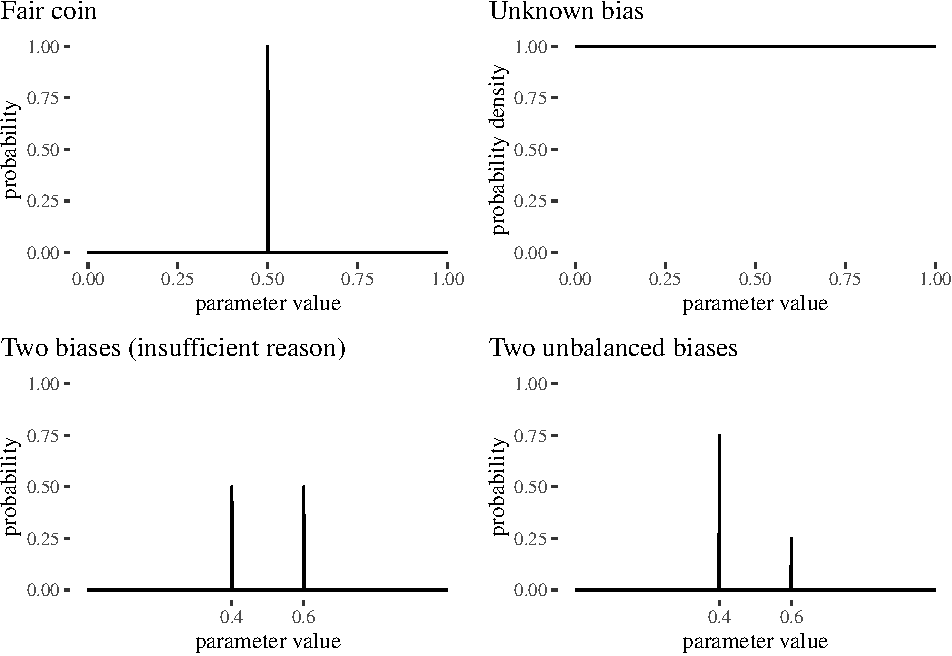
\includegraphics[width=1\linewidth]{chapter-outline_files/figure-latex/fig:evidenceResponse2-1} \end{center}
\caption{Examples of RA's distributions responding to various types of evidence for typical cases brought up in the literature.}



\label{fig:evidenceResponse}
\end{figure}

How is learning about frequencies modeled on this approach, assuming
independence and constant frequency/probability for all the
observations? The Bayes way. You start with some prior density \(p\)
over the parameter values. For instance, if you start with complete lack
of information, \(p\) might be uniform. Then you observe the data \(D\)
which is basically the number of successes \(s\) in a certain number of
observations \(n\). For each particular possible value \(\theta\) of the
parameter, the probability of \(D\) conditional on \(\theta\) follows
the binomial distribution. The probability of \(D\) is obtained by
integration. That is:

\begin{align*}
p(\theta \vert D) & = \frac{p(D\vert \theta)p(\theta)}{p(D)}\\
& = \frac{\theta^s (1-\theta)^{(n - s)}p(\theta)}{\int \theta'^s (1-\theta')^{(n - s)}p(\theta')\,\, d\theta'}
\end{align*}

For instance, belief inertia does not arise. If you just start with a
uniform density over \([0,1]\) as your prior, use binomial probability
as likelihood, observing any non-zero number of heads will exclude 0 and
observing any non-zero number of tails will exclude 1 from the basis of
the posterior, and the posterior distribution becomes more centered
around the parameter estimate as the observations come in. Let's see an
example with a grid approximation (\(n=1k\)) and coin tossing (grid
approximation allows us also to talk about probabilities rather than
densities). Our prior is uniform, and then, in subsequent steps, we
observe heads, another heads, and then tails. This is what happens with
the posterior as we go (Figure \ref{fig:intertia2}).

\begin{figure}[H]

\begin{center}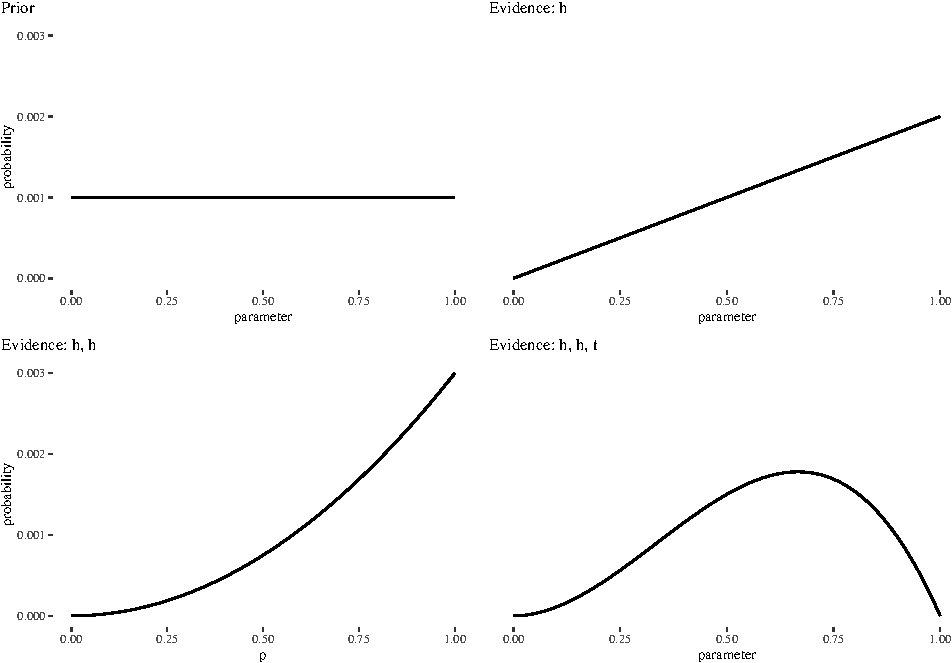
\includegraphics[width=1\linewidth]{chapter-outline_files/figure-latex/fig:inertia3-1} \end{center}
\caption{As observations of heads, heads and tails come in, extreme parameter values drop out of the picture and the posterior is shaped by the evidence.}
\label{fig:intertia2}
\end{figure}

\hypertarget{higher-order-probabilities-and-bayesian-networks}{%
\section{Higher-order probabilities and Bayesian
networks}\label{higher-order-probabilities-and-bayesian-networks}}

The reader might be worried: how can we handle the computational
complexity that comes with moving to higher-order probabilities? The
answer is, as long as we have decent ways of either basing densities on
sensible priors and data, or eliciting densities from experts (CITE
UNCERTAIN JUDMENTS), implementation is not computationally unfeasible,
as we can approximate densities using sampling. To illustrate, let us
start with a simplified BN developed by CITE FENTON to illustrate how
conviction was unjustified in the Clark case (Figure
\ref{fig:scBNplot}). to illustrate a point about the notorious Sally
Clark case (Figure \ref{fig:scBNplot}).\footnote{R. v. Clark (EWCA Crim
  54, 2000) is a classic example of how the lack of probabilistic
  independence between events can be easily overlooked. Sally Clark's
  first son died in 1996 soon after birth, and her second son died in
  similar circumstances a few years later in 1998. At trial, the
  paediatrician Roy Meadow testified that the probability that a child
  from such a family would die of Sudden Infant Death Syndrome (SIDS)
  was 1 in 8,543. Meadow calculated that therefore the probability of
  both children dying of SIDS was approximately 1 in 73 million. Sally
  Clark was convicted of murdering her infant sons (the conviction was
  ultimately reversed on appeal). The calculation illegitimately assumes
  independence, as the environmental or genetic factors may predispose a
  family to SIDS. The winning appeal was based on new evidence: signs of
  a potentially lethal disease---contrary to what was assumed in the
  original case---were found in one of the bodies.} The arrows depict
relationships of influence between variables. \textsf{Amurder} and
\textsf{Bmurder} are binary nodes corresponding to whether Sally Clark's
sons, call them A and B, were murdered. These influence whether signs of
disease (\textsf{Adisease} and \textsf{Bdisease}) and bruising
(\textsf{Abruising} and \textsf{Bbruising}) were present. Also, since
son A died first, whether A was murdered casts some light on the
probability of son B being murdered.

\begin{figure}[H]

\begin{center}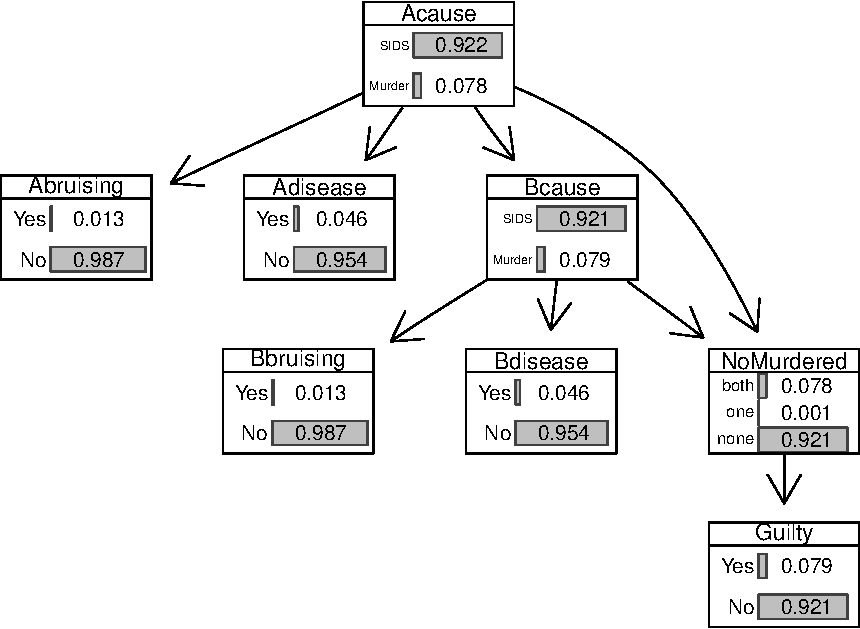
\includegraphics[width=0.8\linewidth]{chapter-outline_files/figure-latex/scBNplot2-1} \end{center}
\caption{The BN developed by FENTON ET AL., with marginal prior probabilities.}
\label{fig:scBNplot}
\end{figure}

The point to be illustrated was that with a sensible choice of
probabilities for the conditional probability tables in the BN,
conviction was not justified at any of the major stages (Figure
\ref{fig:SCfentonTable}).

\begin{figure}

\begin{center}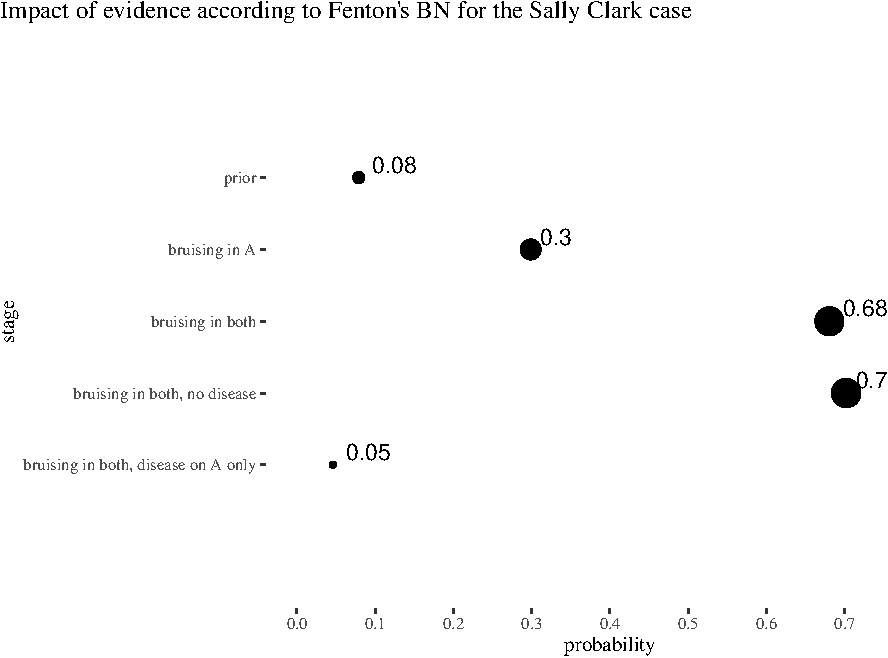
\includegraphics[width=1\linewidth]{chapter-outline_files/figure-latex/SCfentonTable2-1} \end{center}

\caption{The prior and posterior probabilities for Fenton's Sally Clark BN.}

\label{fig:SCfentonTable}

\end{figure}

One reason the reader might worry is that the choice of the
probabilities is fairly specific, and it is not obvious where such
precise values should come from. We have already discussed how frequency
and probability estimates usually come at least with some aleatory
uncertainty around them that cannot be represented by first-order
probabilities. The usual response REFS FOR SENSITIVITY ANALYSIS is that
a range of such selections should be tested, perhaps with special focus
on extreme but still plausible values. We have already discussed how
much care is needed on such approach as it to some extent ignores the
shape of the underlying distributions. Crucially, on the sensitivity
approach different probability measures (or point estimates) are not
distinguished in terms of their plausibility, and so this plausibility
is not accounted for in the analysis. Moreover, if in the sensitivity
analysis the further decision is guided by the results for the extreme
measures, they might be play an undeservedly strong role. {[}STORY ABOUT
MAKING DAILY DECISION THIS WAY TO ILLUSTRATE{]}

Some of these concerns are at least dampened when we deploy the higher
order probabilities in the BN. The general method is as follows. Each
particular node in a precise BN has a probability table determined by a
finite list of numbers. If it's a root node, its probability table is
determined by one number, if it's a node with one parent, its table is
determined by two numbers etc. Now, suppose that instead of precise
numbers we have densities over parameter values for those determining
numbers. Densities of interests can then be approximated by (1) sampling
parameter values from the specified distributions, (2) plugging them
into the construction of the BN, and (3) evaluating the probability of
interest in that precise BN. The list of the probabilities thus obtained
will approximate the density fo interest. In what follows we will work
with sample sizes of 10k. For instance, your conditional probabilities
might look as illustrated in Figure \ref{fig:SCwithHOPa}. One of them is
based on a truncated normal distribution to emphasize that the framework
give us much freedom in the specification of distributions.

\begin{figure}

\begin{center}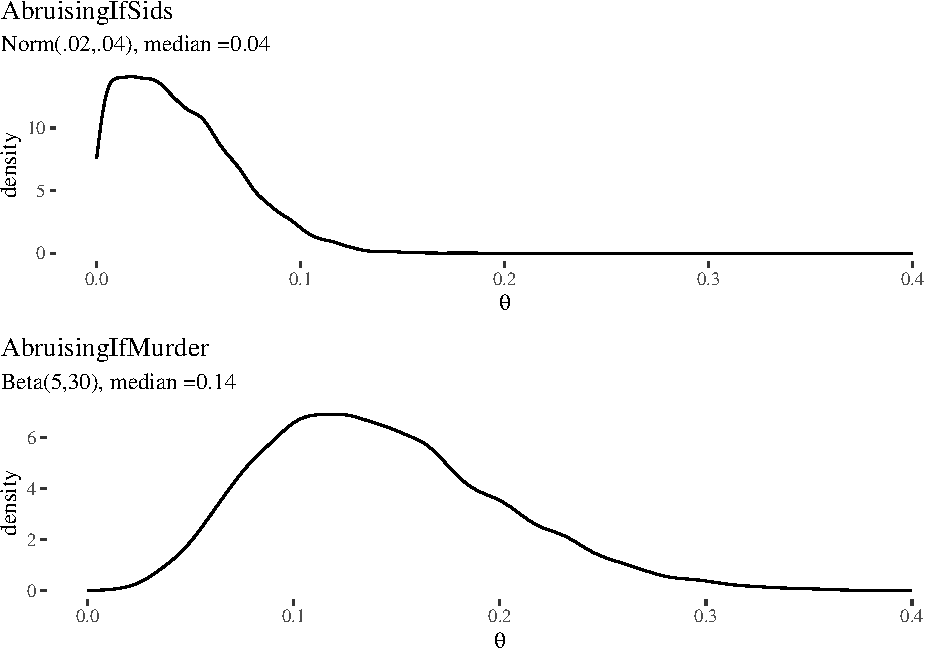
\includegraphics[width=0.9\linewidth]{chapter-outline_files/figure-latex/fig:SCwithHOPa-1} \end{center}

\caption{Example of approximated uncertainties about conditional probabilities in the Sally Clark case.}
\label{fig:SCwithHOPa}
\end{figure}

\begin{figure}

\begin{center}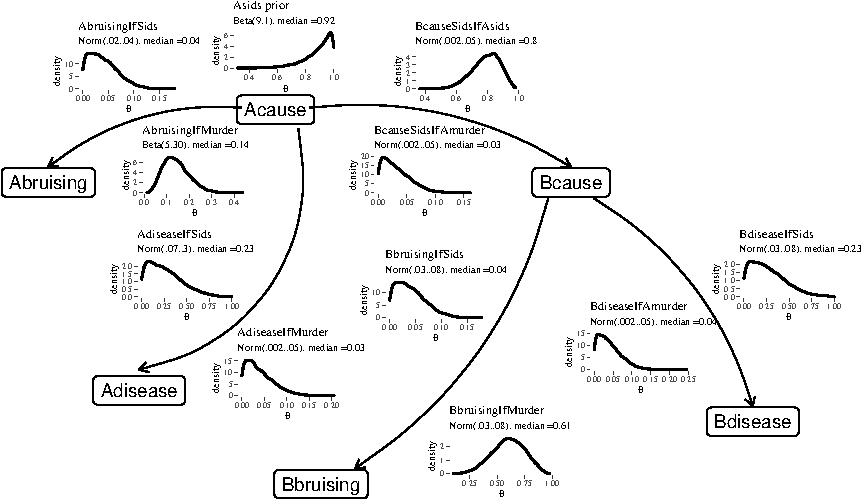
\includegraphics[width=1.6\linewidth,height=2\textheight,angle=90]{chapter-outline_files/figure-latex/SCwithHOP-1} \end{center}

\caption{Example of a HOP approach tor the Sally Clark Case  approximated by sampling probabilities  and constructing 10k BNs.}
\label{fig:SCwithHOP}
\end{figure}

Using these we can investigate the impact of incoming evidence as it
arrives (Figure \ref{fig:SCwithHOP2}). We start with the prior density
for the \s{Guilt} node. Then, we update with the evidence of signs of
bruising in both children. Next, we consider what would have happened if
also both children showed no sign of potentially lethal disease.
Finally, we look at the (simplified) evidential situation at the time of
the appeal: signs of bruising in both children, and signs of lethal
disease discovered in only the first child. One thing to notice that
even in the strongest scenario against Sally Clark (third
visualization), while the median of the posterior distribution was above
.95, the uncertainty around that median is still too wide to legitimize
conviction as the lower limit of the 89\% HPDI is at .83. This
illustrates the idea that taking the point estimates and running with
them might lead to overconfidence, and that paying attention to
uncertainties about the estimates can make an important difference to
our decisions and their accuracy.

\begin{figure}

\begin{center}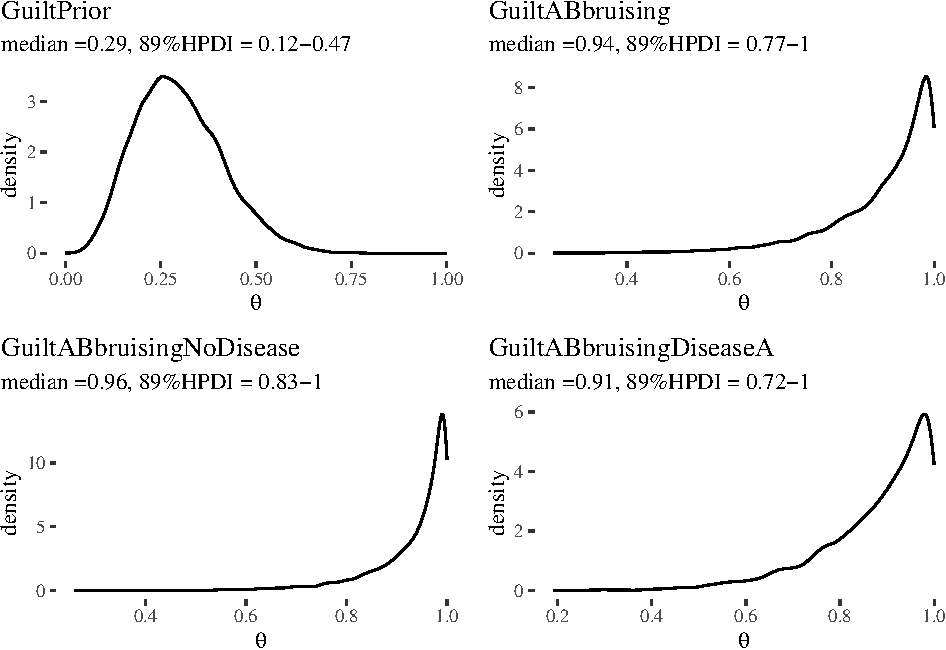
\includegraphics[width=0.9\linewidth]{chapter-outline_files/figure-latex/SCwithHOP2-1} \end{center}


\caption{Impact of incoming evidence in the Sally Clark case.}
\label{fig:SCwithHOP2}
\end{figure}

Moreover, if we are interested in likelihood ratios, the same approach
can be used: sample from the selected distribution appropriate for the
conditional probabilities at hand, then divide the corresponding
samples, obtaining a sample of likelihood ratios, approximating the
density capturing the recommended uncertainty about the likelihood
ratio. For instance, we can use this tool to gauge our uncertainty about
the likelihood ratios corresponding to the signs of bruising in son A
and the presence of the symptomps of a potentially lethal disease in son
A (Figure \ref{fig:SClrs}).

\begin{figure}[H]


\begin{center}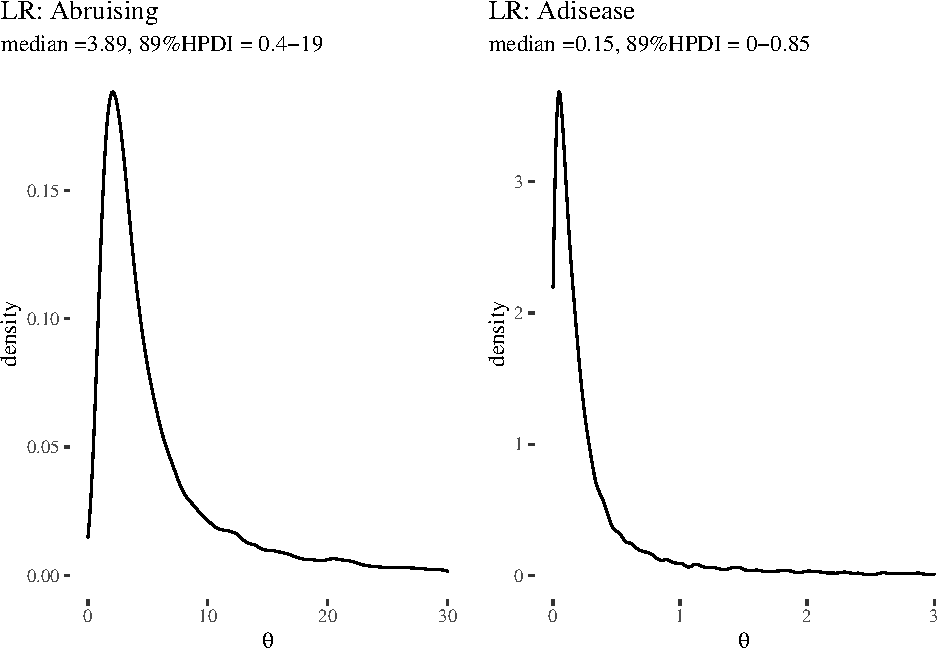
\includegraphics[width=0.9\linewidth]{chapter-outline_files/figure-latex/SClrs-1} \end{center}

\caption{Likelihood ratios forbruising and signs of disease in child A in the Sally Clark case.}
\label{fig:SClrs}

\end{figure}

\todo{Discuss the negation problem?}

\hypertarget{weight-of-evidence}{%
\section{Weight of evidence}\label{weight-of-evidence}}

\todo{Yeh, I think in the end this will be another chapter}

The chapter now turns to the weight of evidence and its formalization.

\textbf{Comment:} It is conceptually important to separate the
discussion about precise, imprecise, and higher order probabilism
(previous sections) from weight (this section). Weight of evidence is
one way in which higher order probabilism can be put to use. It can be
confusing to run the discussion of higher order probabilism together
with weight of evidence. Higher order probabilism can still make perfect
sense even if no theory of weight cen be worked out.

\hypertarget{motivating-examples}{%
\subsection{Motivating examples}\label{motivating-examples}}

This section should start with illustrative examples of the
weight/balance distinction and why ``balance alone'' isn't enough to
model the evidential uncertainty relative to a hypothesis of interest.
These examples should be chosen carefully. We can use legal and
non-legal examples. The driving intuition is given by Keynes with the
weight/balance distinction. Some of the examples we saw earlier in
talking about imprecise probabilism can be mentioned here again, such as
(a1) and (a2), and perhaps also (b) and (c).

Upshot is that uncertainty cannot be captured by balance of evidence
alone. There is a further dimension to uncertainty. So we need a theory
that can accommodate this further level of uncertainty. This theory is
essentially the higher order probabilism introduced before.

\hypertarget{desiderata}{%
\subsection{Desiderata}\label{desiderata}}

Here we can discuss monotonicity, completeness, strong increase, etc
(see current \textbf{section 1}). We can list the intuitive properties
(based on the example we presented in both philosophy and law) that any
theory of weight (and perhaps also of completeness/resilience, but on
these notions, see later) should be able to capture. We should try to
keep these requirements as simple as possible and leave complications to
footnotes.

\hypertarget{formal-characterization-of-weight}{%
\subsection{Formal characterization of
weight}\label{formal-characterization-of-weight}}

Higher order probabilism is then put to use to deliver a theory of
weight. What is now in \textbf{section 11} (``Weight of a
distribution'') and \textbf{sections 13} and \textbf{14} ('' Weight of
evidence'' and ``Weights in Bayesian Networks'') forms the bulk of the
theory.

We should also demonstrate that the proposed theory of weight does meet
the intuitive desiderata and can handle the motivating examples. To
better appreciset the novelty of the proposal, It might be interesting
to raise the following questions:

\begin{itemize}

\item[q1] what does a theory of weight based on precise probabilism look like? (maybe it consists of something like Skyrms' resilience or Kaye's completeness, the problem being that these are not measures of weight, but of something else, more on these later)

\item[q2] what does a theory of weight based on imprecise probabilism look like? (is Joyce's theory essentially an attempt to use imprecise probabilism to construct a theory of weight? )\todo{Well, it's a bit funny as Joyce's weight uses precise chance hypotheses instead of IP, so hard to say}

\item[q3] what does a theory of weight based on higher order probabilism look like?

\end{itemize}

Here we are defending a theory fo weight based on higher order
probabilism, but it is interesting to contrast it with a theory of
weight based on the other version of legal probabilism. Here we can also
show why Joyce's theory of weight does not work (either in the main text
or a footnote).

\textbf{Comment:} The current exposition in chapter 11, 13 and 14,
however, is complicated---perhaps overly so. The move from ``weight of a
distribution'' to ``weight of evidence'' is not intuitive and can
confuse the reader. Is there a simpler story to be told here? I think
so. See below.
\todo{Brilliant, I think I can start talking about conditional probabilities to begin with}

\textbf{Suggestion:} There seems to be a nice symmetry. Start with
precise probabilism. We can use sharp probability theory to offer a
theory of the value of the evidence (i.e.~likelihood ratio). Actually, I
think that the likelihood ratio model the idea of balance of the
evidence. What Keynes distinction weight/balance shows is that
likelihood ratio are not, by themselves, enough to model the value of
the evidence. The straightforward move here seems to just have
\textbf{higher order likelihood ratios}. Wouldn't higher order
likelihood ratio be essentially your formal model of the weight of the
evidence? Your measure of weight tracks the difference between (the
weight of the) prior distribution (and the weight of the) posterior
distribution. But higher order likelihood ratios essentially do the same
thing, just like precise likelihood ratios track the difference between
prior and posterior. Is this right? \todo{Yup, more or less}

\textbf{Comment:} If weight if measured by higher order likelihood
ratios, then this can be seen as a generalization of thoughts that many
other had -- say that the absolute value of the likelihood ratio is a
measure of weight (Nance, Glenn Shafer) or that likelihood ratio must be
a measure of weight (Good; see current \textbf{section 4}). So I think
using ````higher order likelihood ratio'' could be a more appealing way
to sell the idea of weight of evidence since most people are already
familiar with likelihood ratios.

\hypertarget{limits-of-our-contribution}{%
\subsection{Limits of our
contribution}\label{limits-of-our-contribution}}

Work by Nance of Dahlman suggests that ``weight'' should play a role in
the standard of proof. We do not take a position on that. Weight could
be regulated by legal rules at the level of rules of decision, rule of
evidence, admissibility, sanctions at the appellate level. All that
matters to us is that, in general, legal decision-making is sensitive to
these further levels of uncertainty (quantity, completeness,
resilience), but whether this should be codified at the level of the
standard of proof or somewhere else, we are not going to take a stance
on that.

\hypertarget{objection}{%
\subsection{Objection}\label{objection}}

Ronald Allen or Bart Verheij might object as follows. Precise
probabilism is bad because we do not always have the numbers we need to
plug into the Bayesian network. Imprecise probabilism partly addresses
this problem by allowing for a range instead of precise numbers. How
does higher order probabilism help address the practical objection that
we often we do not have the numbers we need to plug into the Bayesian
network?

\hypertarget{completeness-and-resilience}{%
\section{Completeness (and
resilience?)}\label{completeness-and-resilience}}

Next the chapter turns to notions related to the weight of evidence,
such as completeness (and perhaps resilience as well). See current
\textbf{sections 5} and \textbf{6}.

\hypertarget{motivating-example}{%
\subsection{Motivating example}\label{motivating-example}}

Give an example using completeness of evidence (pick one or more court
cases). The court case we can use is Porter v. City of San Francisco
(see file with Marcello's
notes).\footnote{This is a wrongful death case in which victim was committed to a hospital facility, but escaped and then died under unclear circumstances. So the nurses and other hospital workers---actually, the city of San Francisco---are accused of contributing to this person's death. Need to check exact accusation---this is not a criminal case. A phone call was made to social services shortly after the person disappeared, but its content was erased from hospital records. Court agrees that content of phone call would be helpful to understand what happened and to assess the credibility of hospital's workers ("The Okupnik call is the only contemporaneous record of what information was reported to the SFSD about Nuriddin’s disappearance, and could contain facts not otherwise known about her disappearance and CCSF’s response. Additionally, the call is relevant to a jury’s assessment of Okupnik’s credibility"). The court thought that the hospital should have kept records of that call. But court did not think the hospital acted in bad faith or intentionally, so it did NOT issue an "adverse inference instruction" (=the missing evidence was favorable to the party that should have preserved it, but failed to do it).}
The jury is given an instruction that a call recording is missing, but
no instruction whether the call should be assumed to be favorable or
not.

What is the jury supposed to do with this information? If the call could
contain information that is favorable or not, shouldn't the jury simply
ignore the fact that the call recording is missing (Hamer's claim)?
Modelling with Bayesian network might turn out useful. Cite also David
Kaye on the issue of completeness. His claim is that when evidence is
known to be missing, then this information should simply be added as
part of the evidence, which is precisely what the court in Porter does.
But again, once we add the fact that the evidence is missing what is the
evidentiary significance of that? What is te jury supposed to do with
that? Does Pr(H) go up, down or stays the same? Kaye does not
say\ldots{}

\hypertarget{bayesian-network-model}{%
\subsection{Bayesian network model}\label{bayesian-network-model}}

\textbf{Comment} I am thinking that incompleteness is modeled by adding
an evidence node to a Bayesian network but without setting a precise
value for that node, and then see if the updated network yields a
different probability than the previous network without the missing
evidence node. The missing evidence node could be added in different
places and this might changes things. In the Porter case the missing
evidence seems to affect the credibility of the other evidence in the
case, we would have a network like this:
\(H\rightarrow E \leftarrow C\), where \(C\) is the missing evidence
node and \(E\) is the available evidence nose. My hunch is that (see
also our paper on reverse Bayesianiam and unanticipated possibilities)
the addition of this credibility node will affect the probability of the
hypothesis (thus proving Hamer wrong).
\todo{I think this will depend on how the probability of obtaining new evidence given guilt and given innocence are, I will keep thinking about this, we'll move to this once the earlier bits are done}

\hypertarget{expected-weight-model}{%
\subsection{Expected weight model}\label{expected-weight-model}}

\textbf{Question:} If what I say above in the comment is correct, then a
question arises, do we need higher order probabilism to model
completeness?

\textbf{Possible answer:} We can use expected weight (see current
\textbf{section 14}). If the expected weight of an additional item of
evidence is null, that would mean that its addition (not matter the
value the added evidence would take) cannot change the probability of
the hypothesis. If the expected weight is different from zero (pace
Hamer who thinks the expected weight is always null), then the evidence
can change the probability of the hypothesis.

\todo{LR ratio and weight}

\hypertarget{weight-and-accuracy}{%
\section{Weight and accuracy}\label{weight-and-accuracy}}

This section addresses the question, why care about weight?

\hypertarget{conclusion}{%
\section*{Conclusion}\label{conclusion}}
\addcontentsline{toc}{section}{Conclusion}

\hypertarget{refs}{}
\begin{CSLReferences}{1}{0}
\leavevmode\vadjust pre{\hypertarget{ref-bradley2012uncertaintyPhD}{}}%
Bradley, S. (2012). \emph{Scientific uncertainty and DecisionMaking}
(PhD thesis). London School of Economics; Political Science.

\leavevmode\vadjust pre{\hypertarget{ref-bradley2019imprecise}{}}%
Bradley, S. (2019). {Imprecise Probabilities}. In E. N. Zalta (Ed.),
\emph{The {Stanford} encyclopedia of philosophy} ({S}pring 2019).
\url{https://plato.stanford.edu/archives/spr2019/entries/imprecise-probabilities/};
Metaphysics Research Lab, Stanford University.

\leavevmode\vadjust pre{\hypertarget{ref-CampbellMoore2020accuracy}{}}%
Campbell-Moore, C. (2020). \emph{Accuracy and imprecise probabilities}.

\leavevmode\vadjust pre{\hypertarget{ref-Carr2020impreciseEvidence}{}}%
Carr, J. R. (2020). Imprecise evidence without imprecise credences.
\emph{Philosophical Studies}, \emph{177}(9), 2735--2758.
\url{https://doi.org/10.1007/s11098-019-01336-7}

\leavevmode\vadjust pre{\hypertarget{ref-Dietrich2016pooling}{}}%
Dietrich, F., \& List, C. (2016). Probabilistic opinion pooling. In A.
Hajek \& C. Hitchcock (Eds.), \emph{Oxford handbook of philosophy and
probability}. Oxford: Oxford University Press.

\leavevmode\vadjust pre{\hypertarget{ref-Lee2017impreciseEpistemology}{}}%
Elkin, L. (2017). \emph{Imprecise probability in epistemology} (PhD
thesis). Ludwig-Maximilians-Universit{ä}t;
Ludwig-Maximilians-Universität München.

\leavevmode\vadjust pre{\hypertarget{ref-Elkin2018resolving}{}}%
Elkin, L., \& Wheeler, G. (2018). Resolving peer disagreements through
imprecise probabilities. \emph{Noûs}, \emph{52}(2), 260--278.
\url{https://doi.org/10.1111/nous.12143}

\leavevmode\vadjust pre{\hypertarget{ref-VanFraassen2006vague}{}}%
Fraassen, B. C. V. (2006). Vague expectation value loss.
\emph{Philosophical Studies}, \emph{127}(3), 483--491.
\url{https://doi.org/10.1007/s11098-004-7821-2}

\leavevmode\vadjust pre{\hypertarget{ref-Gardenfors1982unreliable}{}}%
Gärdenfors, P., \& Sahlin, N.-E. (1982). Unreliable probabilities, risk
taking, and decision making. \emph{Synthese}, \emph{53}(3), 361--386.
\url{https://doi.org/10.1007/bf00486156}

\leavevmode\vadjust pre{\hypertarget{ref-joyce2005probabilities}{}}%
Joyce, J. M. (2005). How probabilities reflect evidence.
\emph{Philosophical Perspectives}, \emph{19}(1), 153--178.

\leavevmode\vadjust pre{\hypertarget{ref-Kaplan1968decision}{}}%
Kaplan, J. (1968). Decision theory and the fact-finding process.
\emph{Stanford Law Review}, \emph{20}(6), 1065--1092.

\leavevmode\vadjust pre{\hypertarget{ref-keynes1921treatise}{}}%
Keynes, J. M. (1921). \emph{A treatise on probability, 1921}. London:
Macmillan.

\leavevmode\vadjust pre{\hypertarget{ref-Levi1974ideterminate}{}}%
Levi, I. (1974). On indeterminate probabilities. \emph{The Journal of
Philosophy}, \emph{71}(13), 391. \url{https://doi.org/10.2307/2025161}

\leavevmode\vadjust pre{\hypertarget{ref-Levi1980enterprise}{}}%
Levi, I. (1980). \emph{The enterprise of knowledge: An essay on
knowledge, credal probability, and chance}. MIT Press.

\leavevmode\vadjust pre{\hypertarget{ref-Mayo-Wilson2016scoring}{}}%
Mayo-Wilson, C., \& Wheeler, G. (2016). Scoring imprecise credences: A
mildly immodest proposal. \emph{Philosophy and Phenomenological
Research}, \emph{92}(1), 55--78.
\url{https://doi.org/10.1111/phpr.12256}

\leavevmode\vadjust pre{\hypertarget{ref-Rinard2013against}{}}%
Rinard, S. (2013). Against radical credal imprecision. \emph{Thought: A
Journal of Philosophy}, \emph{2}(1), 157--165.
\url{https://doi.org/10.1002/tht3.84}

\leavevmode\vadjust pre{\hypertarget{ref-Schoenfield2017accuracy}{}}%
Schoenfield, M. (2017). The accuracy and rationality of imprecise
credences. \emph{Noûs}, \emph{51}(4), 667--685.
\url{https://doi.org/10.1111/nous.12105}

\leavevmode\vadjust pre{\hypertarget{ref-seidenfeld2012forecasting}{}}%
Seidenfeld, T., Schervish, M., \& Kadane, J. (2012). Forecasting with
imprecise probabilities. \emph{International Journal of Approximate
Reasoning}, \emph{53}, 1248--1261.
\url{https://doi.org/10.1016/j.ijar.2012.06.018}

\leavevmode\vadjust pre{\hypertarget{ref-Stewart2018pooling}{}}%
Stewart, R. T., \& Quintana, I. O. (2018). Learning and pooling, pooling
and learning. \emph{Erkenntnis}, \emph{83}(3), 1--21.
\url{https://doi.org/10.1007/s10670-017-9894-2}

\leavevmode\vadjust pre{\hypertarget{ref-Sturgeon2008grain}{}}%
Sturgeon, S. (2008). Reason and the grain of belief. \emph{No{û}s},
\emph{42}(1), 139--165. Retrieved from
\url{http://www.jstor.org/stable/25177157}

\leavevmode\vadjust pre{\hypertarget{ref-walley1991statistical}{}}%
Walley, P. (1991). \emph{Statistical reasoning with imprecise
probabilities}. Chapman; Hall London.

\end{CSLReferences}

\end{document}
